%% IJIS submission draft -- issue #16
%% Ported from docs/paper/draft.md into svjour3 (docs/paper/latex/svjour3.cls
%% + svglov3.clo), the actual LaTeX macro package Springer's own current
%% submission-guidelines page for this journal (10207) links under "LaTeX
%% Package (Download zip, 279 kB)" -- confirmed 2026-08-06 by fetching that
%% page directly (see PROGRESS.md item T1). The earlier sn-jnl-based port
%% was a third-party-corroborated guess and has been replaced.
%%
%% NOT using svepjc3.clo: that class-option file is specific to the
%% European Physical Journal C (a different Springer journal bundled in the
%% same generic zip) and does not apply here. This document uses the
%% generic svglov3.clo per template.tex's plain \documentclass[...]{svjour3}
%% form.
%%
%% Citation style: default svjour3 \cite (no natbib option loaded) produces
%% numbered, compressible bracket citations ([3], [1-3,7]) directly from
%% \@lbibitem / \@citex in svjour3.cls -- this matches the guidelines' own
%% examples exactly, so no natbib/author-year option is used.
%%
%% Bibliography: hand-written \thebibliography (see end of file) rather than
%% BibTeX, since the only .bst shipped in the official zip (spphys.bst) is
%% styled for physics journals, not IJIS, and bibtex is not available in
%% this environment (tectonic only). Each entry is manually formatted to
%% match the guidelines' own reference examples (journal article / article
%% by DOI / online document forms) so no style-file guess is needed. Content
%% (authors/titles/years/DOIs) is unchanged from references.bib, which
%% remains in this directory as the source of truth for that content -- keep
%% both in sync if a reference changes.
%%
%% To build: tectonic ijis-draft.tex
%%
%% Content is otherwise UNCHANGED from the previous sn-jnl port except for
%% one addition: an AI-assistance disclosure subsection in Section 3 (Sect.
%% "Title Page" of the guidelines requires documenting non-copy-editing LLM
%% use in the Methods section; see PROGRESS.md item T1 addendum).
%% Remaining open items are tracked in ../PROGRESS.md.

\RequirePackage{fix-cm}
\documentclass[twocolumn]{svjour3}

\usepackage{graphicx}%
\usepackage{amsmath,amssymb,amsfonts}%
\usepackage{booktabs}%
\usepackage{xcolor}%
\usepackage{textcomp}%
\usepackage{url}% \path{...} for verbatim-safe file/module names (handles _)
\usepackage{tikz}%
\usetikzlibrary{shapes.geometric,arrows.meta,positioning,fit,calc}%

\smartqed

\journalname{International Journal of Information Security}

\begin{document}

\title{A Deterministic Schema Guardrail for LLM-Assisted SOC Alert Triage: A Negative-Result Investigation of Cross-Domain Classifier Transfer}
\titlerunning{A Deterministic Schema Guardrail for LLM-Assisted SOC Alert Triage}

%% TODO before submission: confirm ORCID (optional field on the title page)
%% and any co-author/funding details -- see PROGRESS.md.
\author{Asma Imran}

\institute{Asma Imran \at
  TECIP, Scuola Superiore Sant'Anna, Pisa, Italy \\
  \email{asmaimran2003@gmail.com}
}

\date{Received: date / Accepted: date}

\maketitle

\begin{abstract}
LLM-based Security Operations Center (SOC) copilots increasingly rely on machine-learned guardrails to filter adversarial input before it reaches a triage model. We report a negative result from building and deploying such a guardrail in a real LangGraph-based alert-triage pipeline evaluated on Microsoft's GUIDE dataset. Following a supervisor-suggested design (issue \#10: regex fast-path $\rightarrow$ ML classifier $\rightarrow$ LLM route), we selected a TF-IDF + Logistic Regression detector --- which outperformed Meta's Llama Prompt Guard and Protect AI's LLM Guard on a public jailbreak benchmark (F1 0.883 vs.\ 0.747 and 0.722, respectively, at three orders of magnitude lower latency) --- and integrated it as a second guardrail stage scoped to the \texttt{AlertTitle} field. When evaluated against real GUIDE alert data rather than the benchmark distribution it was selected on, the classifier collapsed to near-chance performance (52.5\% best-case accuracy across a threshold sweep; 1/20 true positives at the best-performing threshold). Root-cause analysis, rather than threshold tuning or retraining, revealed the actual cause: \texttt{AlertTitle} in the real dataset is a closed numeric-ID field (86{,}149 unique integer values), not free text --- the GUIDE schema itself has no free-text column, so no amount of domain-matched training data could have closed the gap. We retired the classifier and replaced it with a deterministic type-validation guardrail that separates classes by construction rather than learned approximation, achieving 100\% accuracy on a balanced synthetic set and zero false positives against 5{,}000 real \texttt{AlertTitle} values. We also report and fix a silent graph-wiring defect this change introduced --- a dead-end node that caused every verdict to default to \texttt{FalsePositive} without raising an error --- and the regression-test suite built to catch it. We argue that correctly diagnosing an unfalsifiable premise, and confirming a mismatch rather than deploying a broken classifier, is itself a reportable contribution for guardrail engineering.
\keywords{SOC triage \and LLM guardrails \and prompt injection \and negative results \and LangGraph \and MITRE ATT\&CK}
\end{abstract}

\section{Introduction}\label{sec1}

\noindent\textbf{Motivation and context.} Security Operations Centers face alert volumes that outpace human triage capacity --- a well-documented driver of analyst alert fatigue \cite{alert_fatigue_survey2026} --- driving interest in LLM copilots that summarize, contextualize, and pre-classify alerts before an analyst sees them (Microsoft Security Copilot \cite{msft_copilot2024}; Ferrag et al.'s cybersecurity-LLM review \cite{ferrag2024}; Srinivas et al.\ \cite{srinivas2025survey}). A recurring design pattern in this space layers a fast, cheap guardrail (regex/keyword filtering) in front of a slower, more capable classifier, which in turn gates access to the LLM itself --- mirroring the layered defense pattern used in general-purpose LLM guardrail frameworks such as Meta's LlamaFirewall \cite{llamafirewall2025} and Llama Prompt Guard \cite{promptguard2024}, and Protect AI's LLM Guard \cite{llmguard2023}.

\noindent\textbf{Problem definition.} This layered pattern assumes the ML classifier stage has a text field to operate on, and that a classifier's benchmark performance is representative of its deployment domain. We show both assumptions can silently fail in a real SOC pipeline: the field a classifier is scoped to may not be free text at all, and a classifier's published F1 score may not transfer to the structured, terse text distribution of real alert data. Discovering this only after deployment --- rather than before, from the schema --- wastes the time-box allocated to a fix that cannot work.

\noindent\textbf{Scope of this work.} We report on a full design-build-evaluate-diagnose cycle carried out inside a working, evaluated LangGraph triage agent over the GUIDE dataset \cite{guide2024}: (1) selecting and integrating a second-stage ML guardrail per a specific architectural suggestion (issue \#10), (2) evaluating it against real data rather than only the benchmark it was selected on, (3) finding it has no usable signal on that data, (4) root-causing \emph{why} rather than retraining, and (5) replacing it with a deterministic guardrail that is provably correct for its target field, hard-gated into the live pipeline. We also report a real reliability defect this change introduced --- a silently dead-ending graph edge --- and the regression-test suite added to prevent recurrence.

\noindent\textbf{Contributions.}
\begin{enumerate}
\item \textbf{A negative-result methodology for guardrail transfer}: we show that a classifier chosen because it wins a public benchmark (F1 0.883 on a chat-style jailbreak eval set) can be statistically indistinguishable from chance on the actual deployment distribution, and we demonstrate that root-causing this from the data schema --- rather than from threshold sweeps or retraining --- is what actually resolves it, in one week instead of an open-ended tuning effort.
\item \textbf{A deterministic schema guardrail} for closed-vocabulary/numeric alert fields, which separates benign input from injection payloads by construction (type validity) rather than by a learned, thresholded score, and is safe to hard-gate for exactly that reason.
\item \textbf{A reliability-engineering finding and fix}: introducing the schema guardrail silently broke the downstream classification routing (a dead-end node LangGraph does not flag at compile time), which a hardcoded default masked as a plausible-looking result instead of a crash. We document the defect, the fix, and the structural regression test (\path{tests/test_graph_wiring.py}) now guarding against recurrence.
\end{enumerate}

\noindent\textbf{Structure of this report.} Section~\ref{sec2} surveys related work in LLM-based SOC copilots, guardrail frameworks, and MITRE ATT\&CK-grounded LLM systems. Section~\ref{sec3} describes the triage pipeline, the MITRE ATT\&CK retrieval stage, and the guardrail decision process in detail. Section~\ref{sec4} reports evaluation results exactly as committed in \path{experiments/results/}. Section~\ref{sec5} discusses the negative-result methodology and limitations. Section~\ref{sec6} concludes.

\section{Related Work}\label{sec2}

\noindent\textit{Base table from \path{docs/literature-review.md}, extended with guardrail-framework and MITRE-grounded-LLM citations found for this paper.}

\noindent\textbf{LLM-based SOC copilots.} Microsoft Security Copilot \cite{msft_copilot2024} demonstrates GPT-4 integrated into commercial SOC workflows, reporting reduced analyst triage time in a closed, proprietary system. Ferrag et al.'s review \cite{ferrag2024} surveys generative-AI/LLM applications across cybersecurity domains --- including intrusion detection, threat intelligence, and malware detection --- situating SOC-alert classification as one of many emerging LLM use cases rather than evaluating a single deployed pipeline against production data, which is the gap this paper's single-pipeline case study addresses. Wei et al.'s CORTEX \cite{cortex2025} is the closest published architecture to ours: a multi-agent, evidence-grounded triage design that reduces false positives relative to single-model baselines, validating our own evidence-grounded (MITRE-context-fetching) LLM node design. Srinivas et al.'s survey \cite{srinivas2025survey} situates human-in-the-loop copilots as the dominant successful pattern in the field, over full automation --- consistent with our pipeline's human-review checkpoint for non-high-confidence verdicts. The GUIDE dataset itself originates from Microsoft's own guided-response research \cite{guide2024}, which we use directly as our evaluation corpus rather than a synthetic or network-flow substitute like CICIDS2017.

\noindent\textbf{Guardrail frameworks for LLM systems.} Meta's LlamaFirewall \cite{llamafirewall2025} and Llama Prompt Guard \cite{promptguard2024}, and Protect AI's LLM Guard \cite{llmguard2023}, are the current reference points for layered LLM input defense --- regex/heuristic fast paths backed by learned classifiers for jailbreak and injection detection. All three are benchmarked, in our own prior work (PR \#12), against a TF-IDF + Logistic Regression baseline on a chat-style jailbreak evaluation set, where the simpler classifier wins on both accuracy and latency. This paper extends that comparison past benchmark accuracy to deployment-distribution transfer, which none of \cite{llamafirewall2025,promptguard2024,llmguard2023} evaluate against structured, SOC-alert-shaped input as opposed to chat-style prompts.

\noindent\textbf{MITRE ATT\&CK-grounded LLM systems.} Recent work grounds LLM threat-intelligence reasoning in MITRE ATT\&CK via retrieval-augmented generation --- e.g., structured retrieval over ATT\&CK technique descriptions to reduce hallucination in attack-technique attribution \cite{rag_cti2025}, knowledge-graph-augmented retrieval over cybersecurity knowledge bases \cite{kgagent2025}, benchmarks for retrieval-augmented LLMs over heterogeneous cyber threat intelligence \cite{cticonnect2025}, and multi-label classification models for tagging free text against ATT\&CK technique taxonomies \cite{mitre_texttag2026} --- a text-tagging task with the same reliance on a free-text input field that Section~\ref{subsec3-3} shows \texttt{AlertTitle} does not have. Freitas et al., who also released the GUIDE dataset \cite{guide2024} this paper evaluates on, separately report an adaptive incident-prioritization system for SOC alert queues at scale \cite{incident_prioritization2026}, underscoring that alert-volume triage remains an active research target beyond this paper's guardrail-specific scope. Our \texttt{fetch\_mitre\_context} pipeline stage (Section~\ref{sec3}) follows the same retrieval-before-classification pattern established by Lewis et al.'s foundational RAG formulation \cite{lewis_rag2020}, applied to MITRE technique context rather than open-domain text.

\noindent\textbf{Prompt injection against structured/agentic input.} Most published prompt-injection taxonomies and defenses target free-text chat or agent-tool input \cite{promptinjection_landscape2026,breaking_defenses2024,llm_privacy_survey2024}. Our contribution is a case study in the opposite direction: a field that looks like it should be defended as text (\texttt{AlertTitle}) is not text at all in the real schema, and the correct defense follows from the schema, not from the injection-detection literature.

\section{Proposed Method}\label{sec3}

\subsection{System architecture}\label{subsec3-1}
The triage pipeline is a \texttt{LangGraph} \texttt{StateGraph} \cite{langgraph2024} (\path{src/agent/graph.py}) over a shared \texttt{AlertState}. Execution order:

\begin{figure*}[h]
\centering
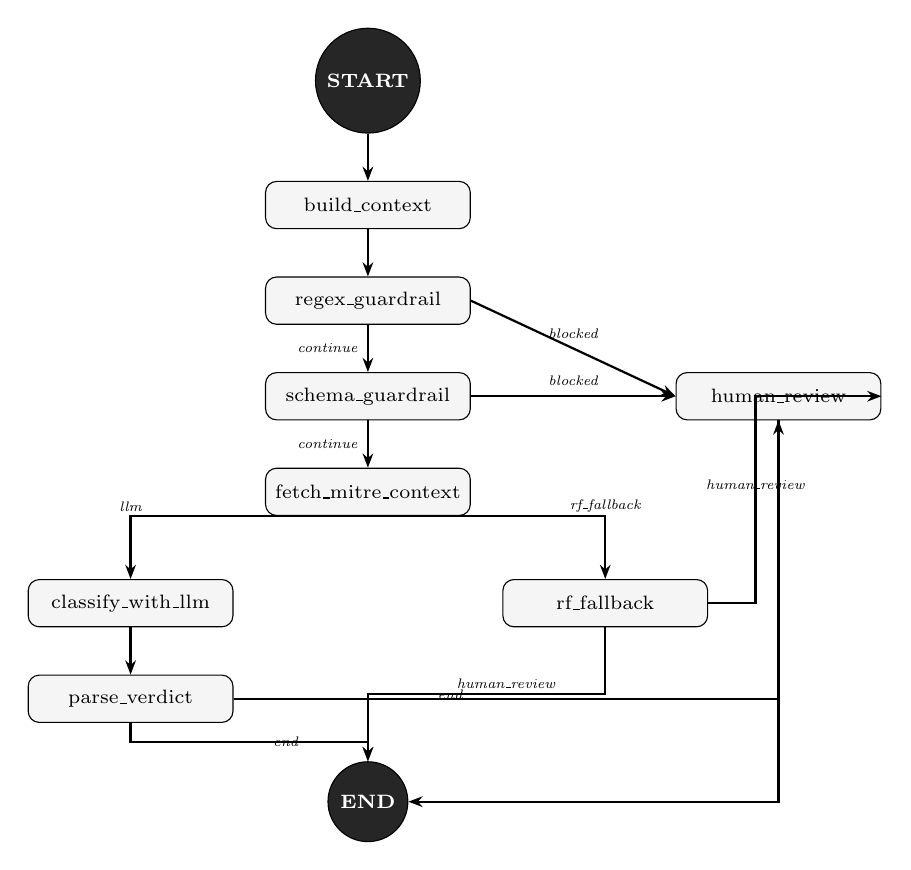
\begin{tikzpicture}[
  node distance=6mm and 10mm,
  every node/.style={font=\scriptsize},
  box/.style={draw, rounded corners, minimum height=6mm, minimum width=26mm, align=center, fill=gray!8},
  term/.style={draw, circle, minimum size=7mm, fill=black!85, text=white, font=\scriptsize\bfseries},
  arr/.style={-{Stealth[length=1.8mm]}, thick},
  lbl/.style={font=\tiny\itshape}
]
\node[term] (start) {START};
\node[box, below=of start] (bc) {build\_context};
\node[box, below=of bc] (rg) {regex\_guardrail};
\node[box, below=of rg] (sg) {schema\_guardrail};
\node[box, below=of sg] (fmc) {fetch\_mitre\_context};
\node[box, below left=8mm and 4mm of fmc] (llm) {classify\_with\_llm};
\node[box, below right=8mm and 4mm of fmc] (rf) {rf\_fallback};
\node[box, below=of llm] (pv) {parse\_verdict};
\node[box, right=26mm of sg] (hr) {human\_review};
\node[term, below=14mm of $(pv)!0.5!(rf)$] (endn) {END};

\draw[arr] (start) -- (bc);
\draw[arr] (bc) -- (rg);
\draw[arr] (rg) -- (sg) node[midway, left, lbl] {continue};
\draw[arr] (rg.east) -- (hr.west) node[midway, above, lbl] {blocked};
\draw[arr] (sg) -- (fmc) node[midway, left, lbl] {continue};
\draw[arr] (sg.east) -- (hr.west) node[midway, above, lbl] {blocked};
\draw[arr] (fmc.south) -| node[pos=0.55, above, lbl] {llm} (llm.north);
\draw[arr] (fmc.south) -| node[pos=0.55, above, lbl] {rf\_fallback} (rf.north);
\draw[arr] (llm) -- (pv);
\draw[arr] (pv.south) |- ($(pv.south)!0.5!(endn.north)$) -| node[near start, left, lbl] {end} (endn.north);
\draw[arr] (pv.east) -| node[near start, above, lbl] {human\_review} (hr.south);
\draw[arr] (rf.south) |- ($(rf.south)!0.5!(endn.north)$) -| node[near start, right, lbl] {end} (endn.north);
\draw[arr] (rf.east) -- ++(6mm,0) |- node[near start, above, lbl] {human\_review} (hr.east);
\draw[arr] (hr.south) |- (endn.east);
\end{tikzpicture}
\caption{Triage pipeline control flow, transcribed directly from the compiled \texttt{StateGraph} in \texttt{src/agent/graph.py}: node names, edges, and conditional-routing labels (\texttt{continue}/\texttt{blocked}, \texttt{llm}/\texttt{rf\_fallback}, \texttt{end}/\texttt{human\_review}) match the routing keys passed to \texttt{add\_conditional\_edges} in the source exactly. Note that the Random Forest fallback path (\texttt{rf\_fallback}) routes directly to \texttt{END}/\texttt{human\_review} without passing through \texttt{parse\_verdict}, unlike the LLM path --- this asymmetry is in the actual graph, not an omission here.}\label{fig1}
\end{figure*}

Two guardrail stages run before any alert reaches the LLM or the MITRE-context retrieval step: a regex fast-path (\texttt{apply\_regex\_guardrail}, pre-existing from Week~7 / issue \#8) and, as of Week~9, a deterministic schema guardrail (\texttt{apply\_schema\_guardrail}) that replaced an ML classifier guardrail evaluated in Week~8. Routing after \texttt{fetch\_mitre\_context} (\texttt{route\_by\_context}) sends alerts with sufficient discriminative context fields to the LLM classifier and sparse alerts to a Random Forest fallback classifier (Week~6). Verdicts below high confidence are routed to a human-review checkpoint rather than ending directly --- the same human-in-the-loop pattern surveyed by \cite{srinivas2025survey}.

\subsection{Data}\label{subsec3-2}
GUIDE \cite{guide2024,guide_kaggle2024}: \path{datasets/GUIDE_train.csv} / \texttt{GUIDE\_Test.csv}, Microsoft's public real-world SOC alert/incident corpus, evaluated on real triage-labeled alerts throughout (not synthetic substitutes). \texttt{AlertTitle}, the field targeted by both guardrail designs in this paper, contains 86{,}149 unique values in the training split, all integers --- confirmed by direct inspection, not inferred from the schema documentation alone.

\subsection{Guardrail decision process --- why the classifier was rejected, not deployed}\label{subsec3-3}

\noindent\textbf{Step 1 --- issue-driven design.} Issue \#10 requested a second-stage ML classifier behind the regex fast-path, citing prior benchmark work comparing Meta Llama Prompt Guard and Protect AI LLM Guard \cite{llamafirewall2025,promptguard2024,llmguard2023}. We pulled that benchmark data and additionally evaluated a TF-IDF + Logistic Regression detector (scikit-learn \cite{pedregosa2011sklearn}), which won on both axes that matter for a gate placed in front of every alert: F1 0.883 vs.\ 0.747 (Prompt Guard) and 0.722 (LLM Guard); median latency 0.79\,ms vs.\ 179\,ms and 183\,ms --- roughly three orders of magnitude faster (\path{experiments/results/} benchmark data referenced in PR \#12).

\noindent\textbf{Step 2 --- integration and a real bug.} The classifier was wired in as \path{src/agent/ml_guardrail.py}, scoped to \texttt{AlertTitle}. Cross-version scikit-learn unpickling (model trained under 1.7.1, environment running 1.7.2) initially produced non-deterministic scores; pinning \texttt{scikit-learn==1.7.1} (later committed to \texttt{requirements.txt} in PR \#14, after an initial local-only fix was caught in review) resolved it.

\noindent\textbf{Step 3 --- deployment-distribution evaluation, not just benchmark evaluation.} Run against real GUIDE alert titles, the detector flagged 100\% of a 9-alert and a 30-alert batch as injection. A single benign sentence (``please schedule a team meeting for next Tuesday'') scored 0.726 against a 0.5 flag threshold. This prompted a purpose-built 40-row SOC-domain evaluation set (\path{experiments/soc_domain_eval_v1.csv}: 20 benign SOC alert titles, 20 injection attempts phrased as alert-field text), scored via \path{experiments/soc_domain_eval.py}.

\noindent\textbf{Step 4 --- a bug inside the negative result.} Initial scoring (PR \#12) had \texttt{score\_text()} reading \texttt{classifier.predict\_proba(X)[0][0]} --- index 0, the benign-class probability --- instead of \texttt{[0][1]}, the injection-class probability the guardrail was meant to threshold on. This inverted the \emph{direction} of every score: the clearest injection example in the eval set (an HTML-comment-style override payload) scored lowest of all 40 rows (0.289), and a mundane benign alert scored highest (0.979). A reviewer (PR \#14) caught the index bug; correcting it flipped both extremes as expected (the same injection example rose to 0.711, the same benign alert fell to 0.021) but did not change the conclusion --- see Section~\ref{sec4}.

\noindent\textbf{Step 5 --- root cause, not retraining.} Before time-boxing a fine-tune of the classifier on SOC-domain-labeled text (the roadmap's original Aug~9 plan), we checked what \texttt{AlertTitle} actually contains. It is a closed numeric-ID field, confirmed against 86{,}149 unique integer values in \texttt{GUIDE\_train.csv}; the GUIDE paper's own alert-dataframe schema lists no free-text categorical column at all. A TF-IDF classifier cannot find linguistic signal in a field that was never linguistic --- no amount of domain-matched retraining data changes that. We retired the fine-tune plan on this basis rather than spending the time-box confirming a predictable failure.

\noindent\textbf{Step 6 --- the correct guardrail, and why it can be hard-gated.} \path{src/agent/schema_guardrail.py} replaces the classifier with \texttt{validate\_field\_types()}: for each field in \texttt{EXPECTED\_NUMERIC\_FIELDS = \{"AlertTitle", "DetectorId"\}}, the value must be an int/float, or a string that parses cleanly as one; anything else --- including any injection payload, which is definitionally not a valid integer --- fails the check. This separates the two classes \emph{by construction}, not by a learned, thresholded approximation, which is precisely why it is safe to hard-gate (\texttt{regex\_guardrail} $\rightarrow$ \texttt{schema\_guardrail} $\rightarrow$ \texttt{fetch\_mitre\_context}, \path{src/agent/graph.py}) in a way the probabilistic ML classifier never was: there is no accuracy/threshold tradeoff to reason about at deployment time.

\subsection{A reliability defect introduced by the fix, and the regression test built to catch it}\label{subsec3-4}
Wiring \texttt{schema\_guardrail} into \texttt{graph.py} deleted the existing conditional edge from \texttt{fetch\_mitre\_context} to \texttt{(classify\_with\_llm | rf\_fallback)} without restoring it. \texttt{LangGraph} does not validate dead-end nodes at compile time, so the graph compiled and ran to completion --- but every alert silently stopped after the MITRE-context lookup, producing no \texttt{predicted\_label}. This was invisible in practice because \texttt{evaluate.py} read the missing key with a default (\texttt{result.get("predicted\_label", "FalsePositive")}) instead of raising, so every alert silently scored as a hardcoded guess rather than crashing or erroring visibly. \path{src/app.py}, \texttt{benchmark.py}, and \texttt{run\_agent.py} all invoke the same compiled graph and were equally affected. No repository test previously existed to catch a structurally dead-ended graph.

The fix restores the deleted conditional edge. \path{tests/test_graph_wiring.py} now asserts, structurally, that every non-END node in the compiled graph has at least one outgoing edge, and separately asserts an end-to-end invocation on a sparse alert produces a real, non-default \texttt{predicted\_label} --- turning this specific bug class into a standing regression check rather than a one-time fix. \path{tests/test_schema_guardrail.py} and \path{tests/test_ml_guardrail.py} similarly convert the manual accuracy spot-checks from Sections~\ref{subsec3-3}--\ref{sec4} into assertions.

\subsection{AI-assistance disclosure}\label{subsec3-5}
An AI coding/writing assistant (Claude, Anthropic) was used throughout this project's development to assist with code implementation, debugging, experiment scripting, and drafting of this manuscript's text, figures, and analysis narrative, under the direct supervision and review of the author. All experimental results, metrics, and claims were independently verified by the author against committed source code and result files before inclusion. The author is accountable for all content and conclusions in this work.

\section{Evaluation}\label{sec4}

\noindent\textit{All figures below are read directly from the named JSON file --- verify against the file before citing in the final version; do not hand-round.}

\subsection{Guardrail classifier selection benchmark (pre-deployment)}\label{subsec4-1}
Source: PR \#12 benchmark table (\texttt{guardrail\_comparison.json} / \texttt{eval\_dataset\_v2.csv}, 1000-row balanced chat-jailbreak eval set --- external to this repo, cited for classifier-selection justification only).

\begin{table*}[h]
\caption{Pre-deployment classifier selection benchmark.}\label{tab1}
\begin{tabular}{@{}lccc@{}}
\toprule
Detector & F1 & Median latency & Throughput \\
\midrule
TF-IDF + Logistic Regression & 0.883 & 0.79\,ms & 1258 alerts/s \\
Meta Llama Prompt Guard      & 0.747 & 179\,ms & 5.6 alerts/s \\
Protect AI LLM Guard         & 0.722 & 183\,ms & 5.5 alerts/s \\
\bottomrule
\end{tabular}
\end{table*}

\subsection{Deployment-distribution evaluation: SOC-domain eval set (post index-bug fix)}\label{subsec4-2}
Source: \path{experiments/results/soc_domain_eval_results.json}, 40-row balanced synthetic set (20 benign / 20 injection), corrected \texttt{[0][1]} scoring.

\begin{table*}[h]
\caption{SOC-domain threshold sweep, post index-bug fix.}\label{tab2}
\begin{tabular}{@{}lcccccccc@{}}
\toprule
Threshold & TP & FP & TN & FN & Accuracy & Precision & Recall & F1 \\
\midrule
0.5  & 3 & 3 & 17 & 17 & 0.500 & 0.500 & 0.15 & 0.231 \\
0.6  & 1 & 1 & 19 & 19 & 0.500 & 0.500 & 0.05 & 0.091 \\
0.7  & 1 & 0 & 20 & 19 & 0.525 & 1.000 & 0.05 & 0.095 \\
0.8  & 0 & 0 & 20 & 20 & 0.500 & 0.000 & 0.00 & 0.000 \\
0.9  & 0 & 0 & 20 & 20 & 0.500 & 0.000 & 0.00 & 0.000 \\
0.95 & 0 & 0 & 20 & 20 & 0.500 & 0.000 & 0.00 & 0.000 \\
\bottomrule
\end{tabular}
\end{table*}

Best achievable accuracy across the sweep is 52.5\% (threshold 0.7), with only 1 of 20 true injections recovered even at that point --- at chance for a balanced set. At threshold $\geq 0.8$ the detector predicts ``injection'' for essentially no input, regardless of true label. This is presented as evidence of \emph{no usable signal} on this domain, not a miscalibration recoverable by threshold tuning.

\begin{figure*}[h]
\centering
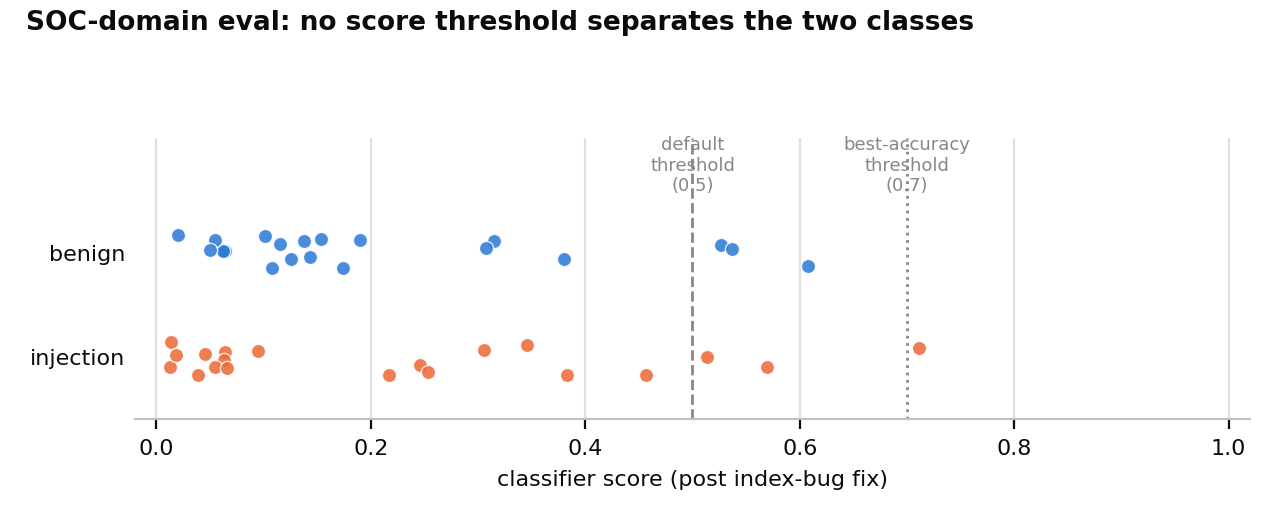
\includegraphics[width=0.72\textwidth]{../figures/score_distribution.png}
\caption{Per-alert classifier scores from \texttt{soc\_domain\_eval\_results.json} (all 40 rows), split by true label. The two classes overlap almost completely across the full score range --- visual confirmation that Table~\ref{tab2}'s threshold sweep fails because there is no threshold to find, not because the sweep stopped short. Generated by \texttt{docs/paper/figures/generate\_figures.py} directly from the committed JSON.}\label{fig2}
\end{figure*}

\subsection{Schema guardrail evaluation (replacement)}\label{subsec4-3}
Source: \path{experiments/results/schema_guardrail_eval.json}, generated by \path{experiments/schema_guardrail_eval.py} (added for this paper).

\begin{itemize}
\item Synthetic (20 benign numeric IDs vs.\ the 20 injection strings from the eval set above): \textbf{100\% accuracy}, 0 false positives, 0 false negatives --- reproduced independently of the PR \#15 description.
\item Real data (5{,}000 \texttt{AlertTitle} values sampled from \texttt{GUIDE\_train.csv}, in row order --- not randomly sampled): \textbf{0 false positives out of 5{,}000}, reproduced independently of the PR \#15 description. \path{experiments/results/schema_guardrail_eval.json} now records \texttt{"status": "ran"}, \texttt{"n\_sampled": 5000}, \texttt{"n\_false\_positives": 0}. Both halves of the guardrail's headline claim now trace to a committed, reproducible artifact rather than PR prose.
\end{itemize}

\subsection{Random Forest baseline}\label{subsec4-4}
Source: \path{experiments/results/baseline_metrics.json} (\texttt{n\_train=79580}, \texttt{n\_test=19895}, \texttt{random\_state=42}).

\begin{table*}[h]
\caption{Random Forest baseline metrics.}\label{tab3}
\begin{tabular}{@{}lc@{}}
\toprule
Metric & Value \\
\midrule
Accuracy            & 0.7718 \\
Macro F1            & 0.7505 \\
BenignPositive F1    & 0.8066 \\
FalsePositive F1    & 0.6561 \\
TruePositive F1      & 0.7889 \\
\bottomrule
\end{tabular}
\end{table*}

\subsection{End-to-end agent evaluation, post graph-wiring fix}\label{subsec4-5}
Source: \path{experiments/results/agent_metrics_post_graph_fix_week9.json} (sample size 30).

\begin{table*}[h]
\caption{End-to-end agent evaluation, post graph-wiring fix ($n=30$).}\label{tab4}
\begin{tabular}{@{}lc@{}}
\toprule
Metric & Value \\
\midrule
Accuracy & 0.5333 \\
Macro F1 & 0.5337 \\
RF baseline (same file, for comparison) & acc 0.7718, F1 0.7505 \\
\bottomrule
\end{tabular}
\end{table*}

Predictions spread across all three classes post-fix (12 BenignPositive / 10 TruePositive / 8 FalsePositive; 9 alerts routed via LLM, 21 via RF fallback) --- the qualitative signal that the graph is classifying again rather than collapsing to a single default.

\noindent\textbf{On the larger \texttt{agent\_metrics\_real\_v3.json} (n=300, accuracy 0.28, macro F1 0.1836) reported elsewhere in the repository history:} this number is not a discrepancy to reconcile against the figure above --- it is from a structurally different, earlier pipeline and is not comparable. Tracing \texttt{experiments/results/agent\_metrics\_real\_v3.json} through \texttt{git log --diff-filter=A} shows it was generated in Week 5 (commit \texttt{d42e41a}/PR \#5), before the sparse-alert RF-fallback route existed (added Week 6, PR \#8) and before the schema guardrail and graph-wiring fix described in Sections~\ref{subsec3-3}--\ref{subsec3-4} (Week 8--9, PRs \#12/\#14/\#15/\#17) --- i.e., against an agent with no fallback for sparse alerts and none of this paper's contributions. Its embedded ``RF baseline: acc=0.374, f1=0.296'' comparison is not a bug either: \texttt{git show d42e41a:experiments/results/baseline\_metrics.json} confirms the baseline model at that point was trained on \texttt{n\_train=6{,}400} rows and genuinely scored 0.374/0.296 --- it was retrained on the full split (\texttt{n\_train=79{,}580}, scoring 0.7718/0.7505, matching Section~\ref{subsec4-4}) only in the Week 9 fix (\texttt{ad02c85}). The comparison number baked into \texttt{real\_v3.json} was accurate for the pipeline and baseline that existed when it was generated; it simply predates almost every contribution this paper describes. \texttt{agent\_metrics\_post\_graph\_fix\_week9.json} (n=30) is therefore the only evaluation run against both the current pipeline and the current baseline, and is the number used in this paper --- its small sample size is retained as an honest limitation (Section~\ref{sec5}) rather than papered over by citing a larger but non-comparable number. A fresh, larger post-fix run was not performed for this paper: it requires a live \texttt{GROQ\_API\_KEY} and the (gitignored) \texttt{baseline\_model.joblib} artifact, neither available in the environment this section was written in.

\subsection{Scalability benchmark}\label{subsec4-6}
Source: \path{experiments/results/week7_scalability_benchmark.json}. Regex guardrail microbenchmark: mean check time 3.766\,\textmu s/alert over 10{,}000 iterations; 10{,}000/10{,}000 injection alerts blocked, 0/10{,}000 benign alerts blocked (at that stage's test set).

The benchmark sweeps three pipeline modes (LLM-only, RF-only, and the hybrid router of Section~\ref{subsec3-3}) across three prompt counts (30/60/120, drawn from the same cached balanced sample, \texttt{guide\_balanced\_40\_per\_class\_seed\_42.csv}) and two worker counts (1, 4).

\begin{table*}[h]
\caption{Scalability benchmark, LLM-only mode.}\label{tab5}
\begin{tabular}{@{}ccccccc@{}}
\toprule
Prompts & Workers & Alerts/s & Mean latency & Accuracy & Macro F1 & Errors \\
\midrule
30  & 1 & 0.5672 & 1.7629\,s & 0.4333 & 0.2016 & 0 \\
30  & 4 & 0.3736 & 2.6765\,s & 0.4333 & 0.2016 & 0 \\
60  & 1 & 0.3705 & 2.6991\,s & 0.3333 & 0.2765 & 0 \\
60  & 4 & 0.3711 & 2.6946\,s & 0.3333 & 0.2765 & 0 \\
120 & 1 & 0.3665 & 2.7284\,s & 0.4000 & 0.3727 & 0 \\
120 & 4 & 0.3756 & 2.6622\,s & 0.3983 & 0.3656 & 2 \\
\bottomrule
\end{tabular}
\end{table*}

Throughput and latency are dominated by remote Groq inference and network round-trips, not local compute --- \texttt{workers=4} gives no consistent speedup over \texttt{workers=1} because Groq's per-minute token budget is shared across threads regardless of worker count. The two errors at 120 prompts/4 workers are rate-limit failures on the live endpoint, not a pipeline defect.

\begin{table*}[h]
\caption{Scalability benchmark, RF-only mode.}\label{tab6}
\begin{tabular}{@{}ccccccc@{}}
\toprule
Prompts & Workers & Alerts/s & Mean latency & Accuracy & Macro F1 & Core util \% \\
\midrule
30  & 1 & 16.69 & 0.060\,s & 0.633 & 0.622 & 10.43 \\
30  & 4 & 41.85 & 0.024\,s & 0.633 & 0.622 & 14.23 \\
60  & 1 & 20.45 & 0.049\,s & 0.700 & 0.490 & 10.41 \\
60  & 4 & 37.70 & 0.027\,s & 0.700 & 0.490 & 14.04 \\
120 & 1 & 29.75 & 0.034\,s & 0.675 & 0.673 & 10.76 \\
120 & 4 & 39.01 & 0.026\,s & 0.675 & 0.673 & 14.16 \\
\bottomrule
\end{tabular}
\end{table*}

Zero errors across all six runs. Local, CPU-bound inference scales the way LLM-only does not: throughput roughly 2--2.5x from 1 to 4 workers at every prompt count, with per-core utilization climbing modestly (10.4\% $\to$ 14.1\%) rather than saturating, since the balanced samples are small relative to the machine's 8 logical cores.

\begin{table*}[h]
\caption{Scalability benchmark, hybrid (context-richness router) mode.}\label{tab7}
\begin{tabular}{@{}ccccccc@{}}
\toprule
Prompts & Workers & Alerts/s & Mean latency & Accuracy & Macro F1 & Routing (RF / LLM) \\
\midrule
30  & 1 & 10.38 & 0.096\,s & 0.633 & 0.259 & 25 / 5 \\
30  & 4 & 6.09  & 0.164\,s & 0.633 & 0.259 & 25 / 5 \\
60  & 1 & 1.76  & 0.567\,s & 0.667 & 0.466 & 47 / 13 \\
60  & 4 & 1.63  & 0.613\,s & 0.667 & 0.466 & 47 / 13 \\
120 & 1 & 1.86  & 0.537\,s & 0.617 & 0.614 & 97 / 23 \\
120 & 4 & 1.88  & 0.533\,s & 0.617 & 0.614 & 97 / 23 \\
\bottomrule
\end{tabular}
\end{table*}

Zero errors across all six hybrid runs. The RF/LLM routing split (83\%, 78\%, 81\% to the RF fallback) is stable across prompt counts and matches the Week~6 baseline of 81.3\%, confirming the context-richness routing logic behaves consistently at scale. Latency tracks the proportion of alerts routed to the LLM rather than prompt count directly --- the 30-prompt run is fastest despite being the smallest sample because proportionally fewer of its alerts hit the LLM path --- and, as with the LLM-only results, \texttt{workers=4} gives no real throughput gain over \texttt{workers=1} (it is measurably slower at 30 prompts) for the same shared-rate-limit reason.

\begin{figure*}[h]
\centering
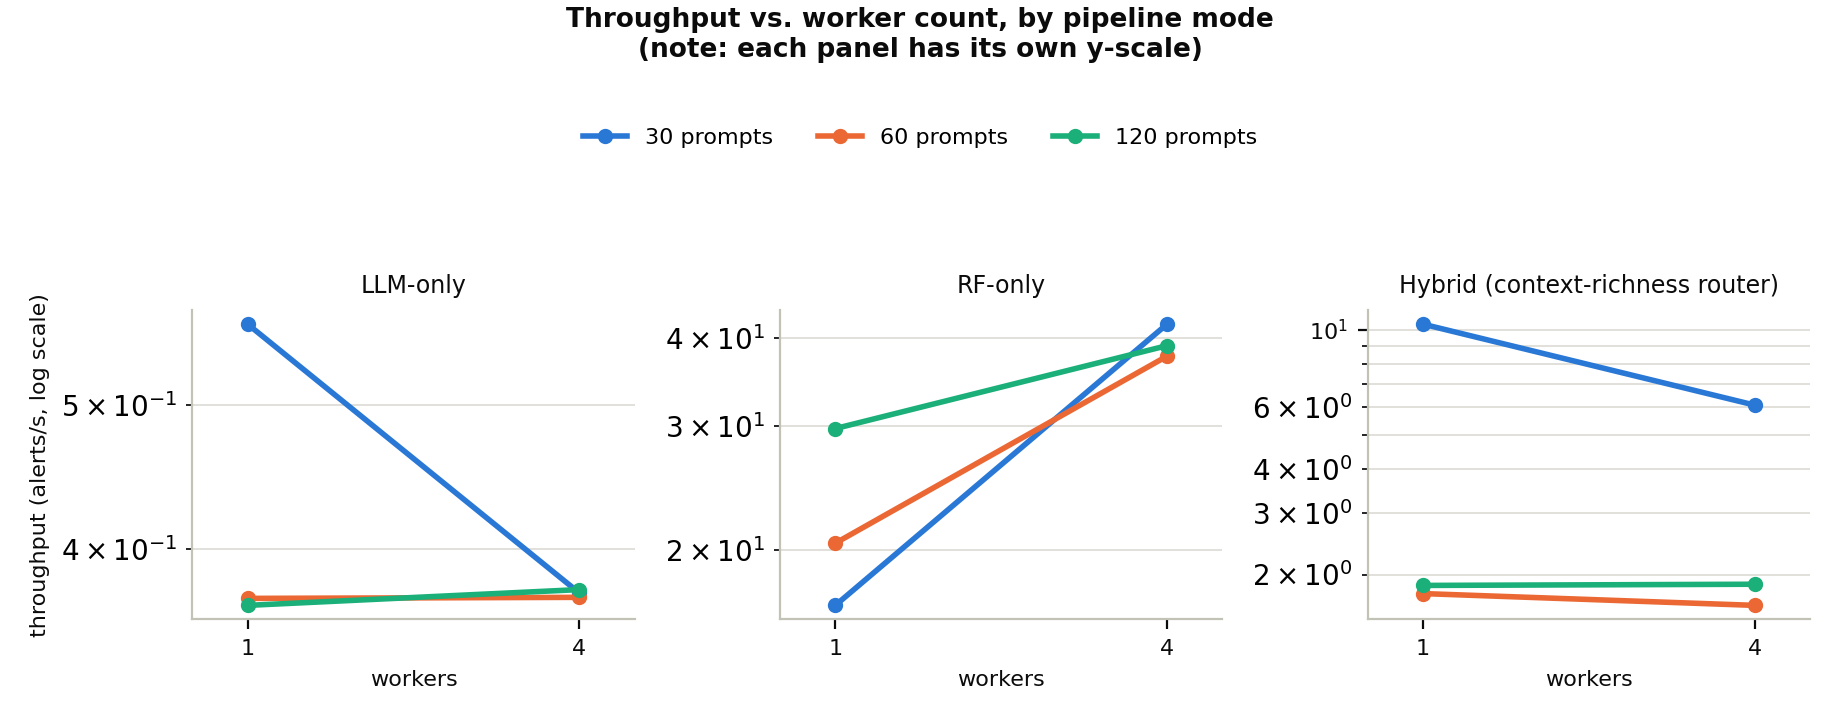
\includegraphics[width=\textwidth]{../figures/throughput_scaling.png}
\caption{Throughput vs.\ worker count, faceted by pipeline mode (note each panel has its own log-scale y-axis --- the three modes differ by roughly two orders of magnitude and are not comparable on a shared axis). RF-only throughput scales with worker count as expected for local CPU-bound inference; LLM-only and hybrid do not, because Groq's per-minute token budget is shared across worker threads regardless of concurrency. Generated by \texttt{docs/paper/figures/generate\_figures.py} directly from \texttt{week7\_scalability\_benchmark.json}.}\label{fig3}
\end{figure*}

\noindent\emph{Full per-run CPU/memory fields --- process CPU seconds, peak RSS --- are in the source JSON but omitted here for brevity; not needed to support the throughput/accuracy claims made in this section or in Section~\ref{sec5}.}

\section{Discussion}\label{sec5}

\noindent\textbf{The negative-result methodology, and why it matters more than a working-but-wrong classifier.} A classifier that appears to work --- because it was evaluated only on the benchmark distribution it was selected against --- is a worse outcome for a production guardrail than one that is honestly shown not to work on the deployment distribution. Section~\ref{subsec4-1} shows the TF-IDF classifier winning decisively against two established guardrail frameworks; had that benchmark result alone been used to justify deployment, the guardrail would have shipped in a state indistinguishable from random on real input (Section~\ref{subsec4-2}), silently passing roughly half of actual injection attempts while also blocking legitimate alerts. The distinction argued in this paper is not ``domain mismatch exists'' --- a known risk in ML deployment generally --- but that \emph{diagnosing it correctly} (checking the schema before retraining) converts an open-ended, unbounded tuning problem into a one-week, closed investigation with a deterministic replacement. Section~\ref{subsec3-3}, Step 5 is the paper's central methodological claim.

\noindent\textbf{The graph-wiring defect as a reliability-engineering contribution.} Section~\ref{subsec3-4}'s defect is notable less for its mechanism (a deleted graph edge) than for how it failed: silently, past a compiled graph, past a running pipeline, into a hardcoded default that looked like a real (if pessimistic) classification. No exception, log line, or crash surfaced it; it was only caught by an independent post-merge audit, not by the change's own review. We argue this is a generalizable risk for any LangGraph-style pipeline where a downstream consumer applies a lenient default to a missing key --- the failure mode is structurally identical to an ML guardrail that silently returns a plausible-but-wrong score, and the fix (a structural graph-completeness test, not just a functional one) generalizes past this specific bug.

\subsection*{Limitations}
\begin{itemize}
\item The SOC-domain evaluation set (Section~\ref{subsec4-2}) is a 40-row synthetic set, not a labeled real-world injection corpus against structured alert fields --- no such public corpus was identified during this work (see Related Work, Prompt injection paragraph).
\item The end-to-end agent evaluation sample used in this paper (Section~\ref{subsec4-5}, n=30) is small relative to the GUIDE test split. It is the only committed run against the current pipeline and current RF baseline; larger historical runs (e.g. \texttt{agent\_metrics\_real\_v3.json}, n=300) predate this paper's contributions (no RF fallback, no schema guardrail) and are not usable as a larger-sample substitute, per the tracing in Section~\ref{subsec4-5}. A larger post-fix run would strengthen this section but requires a live LLM API key and the retrained RF artifact, neither available while writing this draft.
\item The real-data schema-guardrail sample (Section~\ref{subsec4-3}) is the first 5{,}000 rows of \texttt{GUIDE\_train.csv} in file order, not a random sample --- row order in the source file is not known to be free of systematic bias (e.g., chronological or org-clustered ordering), so this should be read as ``no false positives in the first 5{,}000 rows encountered'' rather than a claim about the full 86{,}149-value population.
\item \texttt{EXPECTED\_NUMERIC\_FIELDS} includes \texttt{DetectorId} on the basis of the GUIDE paper's schema description rather than the same direct large-sample inspection applied to \texttt{AlertTitle}; the module docstring notes this as confirmed but the inspection methodology is less thorough than \texttt{AlertTitle}'s.
\item The guardrail-selection benchmark (Section~\ref{subsec4-1}) is drawn from an eval set built for a companion project's chat-jailbreak use case, not this project's SOC-alert domain --- which is exactly the mismatch this paper reports, but it also means Section~\ref{subsec4-1}'s numbers cannot be used as evidence about SOC-domain performance, only as the justification for which classifier was worth testing further.
\end{itemize}

\section{Conclusion}\label{sec6}

We built, evaluated, and rejected a second-stage ML guardrail for an LLM-assisted SOC triage pipeline after confirming --- through direct inspection of the deployment data rather than threshold tuning --- that its target field is not the kind of data the classifier can ever operate on. We replaced it with a deterministic schema guardrail that is correct by construction for that field and safe to hard-gate, unlike the probabilistic classifier it replaced. In fixing the schema guardrail's integration, we found and fixed a silent graph-wiring defect that had been masking every verdict as a default classification, and built a structural regression test suite to prevent recurrence. We argue the central contribution is methodological: correctly diagnosing why a plan cannot work, before spending the time-box that would have confirmed it empirically, is itself a reportable and reusable result for guardrail engineering in structured-data domains.

\section*{Statements and Declarations}

\begin{itemize}
%% TODO before submission: confirm each of these against PROGRESS.md --
%% funding source, competing interests, and data/code availability all
%% still need explicit author confirmation, not just an inherited default.
\item Funding: Not applicable.
\item Conflict of interest/Competing interests: The authors have no competing interests to declare that are relevant to the content of this article.
\item Ethics approval: Not applicable.
\item Consent to participate: Not applicable.
\item Consent for publication: Not applicable.
\item Availability of data and materials: GUIDE dataset \cite{guide2024,guide_kaggle2024}, publicly available from Microsoft. Evaluation result files committed under \path{experiments/results/} in the project repository.
\item Code availability: \url{https://github.com/AI-Security-Internships-2026/02-soc-copilot-threat-analysis}
\item Authors' contributions: Not applicable (single author).
\end{itemize}

\begin{thebibliography}{99}

\bibitem{msft_copilot2024}
Microsoft Security Team: Microsoft Security Copilot. Industry tool (2024). \url{https://www.microsoft.com/en-us/security/business/ai-machine-learning/microsoft-copilot-for-security}

\bibitem{ferrag2024}
Ferrag, M.A., Alwahedi, F., Battah, A., Cherif, B., Mechri, A., Tihanyi, N., Bisztray, T., Debbah, M.: Generative AI in Cybersecurity: A Comprehensive Review of LLM Applications and Vulnerabilities. arXiv preprint arXiv:2405.12750 (2024)

\bibitem{cortex2025}
Wei, B., Tay, Y.S., Liu, H., Pan, J., Luo, K., Zhu, Z., Jordan, C.: CORTEX: Collaborative LLM Agents for High-Stakes Alert Triage. arXiv preprint arXiv:2510.00311 (2025)

\bibitem{srinivas2025survey}
Srinivas, S., Kirk, B., Zendejas, J., Espino, M., Boskovich, M., Bari, A., Dajani, K., Alzahrani, N.: AI-Augmented SOC: A Survey of LLMs and Agents for Security Automation. Journal of Cybersecurity and Privacy 5(4), 95 (2025). \url{https://doi.org/10.3390/jcp5040095}

\bibitem{llamafirewall2025}
Chennabasappa, S., Nikolaidis, C., Song, D., Molnar, D., Ding, S., Wan, S., Whitman, S., Deason, L., Doucette, N., Montilla, A., Gampa, A., de Paola, B., Gabi, D., Crnkovich, J., Testud, J.-C., He, K., Chaturvedi, R., Zhou, W., Saxe, J.: LlamaFirewall: An Open Source Guardrail System for Building Secure AI Agents. arXiv preprint arXiv:2505.03574 (2025)

\bibitem{promptguard2024}
Meta AI: Llama Prompt Guard --- Model Card (2024). \url{https://github.com/meta-llama/PurpleLlama/blob/main/Prompt-Guard/MODEL_CARD.md}

\bibitem{llmguard2023}
Protect AI: LLM Guard --- The Security Toolkit for LLM Interactions. Open-source software (2023). \url{https://github.com/protectai/llm-guard}

\bibitem{guide2024}
Freitas, S., Kalajdjieski, J., Gharib, A., McCann, R.: AI-Driven Guided Response for Security Operation Centers with Microsoft Copilot for Security. arXiv preprint arXiv:2407.09017 (2024)

\bibitem{rag_cti2025}
Alhuzali, A.: LLM-powered threat intelligence: a retrieval-augmented generation approach for cyber attack investigation. PeerJ Computer Science 11, e3371 (2025). \url{https://doi.org/10.7717/peerj-cs.3371}

\bibitem{kgagent2025}
Yang, L., Zhu, H., Mu, J., Li, Q.: KGAgent4CTI: unlocking the power of LLM in threat intelligence. Cybersecurity 9(1), 76 (2026). \url{https://doi.org/10.1186/s42400-025-00458-2}

\bibitem{cticonnect2025}
Cheng, Y., Liu, Y., Li, C., Song, D., Gao, P.: CTIConnect: A Benchmark for Retrieval-Augmented LLMs over Heterogeneous Cyber Threat Intelligence. arXiv preprint arXiv:2510.11974 (2025)

\bibitem{lewis_rag2020}
Lewis, P., Perez, E., Piktus, A., Petroni, F., Karpukhin, V., Goyal, N., K\"uttler, H., Lewis, M., Yih, W., Rockt\"aschel, T., Riedel, S., Kiela, D.: Retrieval-Augmented Generation for Knowledge-Intensive NLP Tasks. In: Advances in Neural Information Processing Systems (NeurIPS) (2020)

\bibitem{promptinjection_landscape2026}
Wang, P., Li, X., Xiang, C., Zhang, J., Li, Y., Zhang, L., Wang, X., Tian, Y.: The Landscape of Prompt Injection Threats in LLM Agents: From Taxonomy to Analysis. arXiv preprint arXiv:2602.10453 (2026)

\bibitem{breaking_defenses2024}
Chowdhury, A.G., Islam, M.M., Kumar, V., Shezan, F.H., Kumar, V., Jain, V., Chadha, A.: Breaking Down the Defenses: A Comparative Survey of Attacks on Large Language Models. arXiv preprint arXiv:2403.04786 (2024)

\bibitem{llm_privacy_survey2024}
Das, B.C., Amini, M.H., Wu, Y.: Security and Privacy Challenges of Large Language Models: A Survey. arXiv preprint arXiv:2402.00888 (2024)

\bibitem{langgraph2024}
LangChain: LangGraph: Multi-Agent Workflows / Agent Orchestration Framework. Software, released January 2024. \url{https://www.langchain.com/langgraph}

\bibitem{mitre_texttag2026}
Crossman, A., Dodd, J., Kumar, V.R.C., Mohammed, R., Plummer, A.R., Sekharudu, C., Warrier, D., Yekrangian, M.: Constructing Multi-label Hierarchical Classification Models for MITRE ATT\&CK Text Tagging. arXiv preprint arXiv:2601.14556 (2026)

\bibitem{incident_prioritization2026}
Freitas, S., Gharib, A., Magenheim, M.: Adaptive Incident Prioritization for Security Operations at Scale. arXiv preprint arXiv:2607.16963 (2026)

\bibitem{alert_fatigue_survey2026}
Ndichu, S., Ban, T., Ozawa, S., Takahashi, T., Inoue, D.: AI-Driven Security Alert Screening and Alert Fatigue Mitigation in Security Operations Centers: A Survey. arXiv preprint arXiv:2605.08316 (2026)

\bibitem{pedregosa2011sklearn}
Pedregosa, F., Varoquaux, G., Gramfort, A., Michel, V., Thirion, B., Grisel, O., Blondel, M., Prettenhofer, P., Weiss, R., Dubourg, V., Vanderplas, J., Passos, A., Cournapeau, D., Brucher, M., Perrot, M., Duchesnay, \'E.: Scikit-learn: Machine Learning in Python. Journal of Machine Learning Research 12, 2825--2830 (2011)

\bibitem{guide_kaggle2024}
Microsoft: Microsoft Security Incident Prediction (GUIDE dataset). Kaggle dataset (2024). \url{https://www.kaggle.com/datasets/Microsoft/microsoft-security-incident-prediction}

\end{thebibliography}

\end{document}
